\documentclass[head=13.6pt]{cce2014-design}
\svnInfo $Id$

% Document details
\title{Design Document: Group 5}
\author{Akram Sharara, Antoni Marek Skoć, Daniel Agius}
\date{31 May 2025}

\begin{document}

\maketitle

\abstract{
As a record of the development of the Morse code receiver, this design document provides an outline of the aims and objectives of the project as set out in the handbook and how they were realized. It discusses a comprehensive view of the development stages of the receiver using figures \ref{generaldiag},\ref{FSM}, and how signal sampling will be handled to convert analog audio inputs to digital ones. A working implementation was finalized in May based on the FSM in fig. 2, with noise handling capabilities and the ability to decode inputs at various transmission speeds, up to even 270 WPM. The receiver can handle inputs with inaccurate timings thanks to an average-based threshold decoding. An LED was used as a digital output to indicate whether the input signal is 1 or 0. A Morse binary tree is used to decode the input, and the input is displayed using a tailor-made function that allows for scrollability for long strings. Testing was done before modification to meet additional requirements as set out in the handbook.
}
\section{Introduction}
The objective of this assignment was to design and implement a microcontroller-based system that receives an input Amplitude Shift Keyed (ASK) Morse code signal, translates it into characters, and displays it on an LCD. Additionally, our implementation of the Morse code translator took into consideration the possible presence of noise in the signal, as well as adapting to different transmission speeds. All code was written in C, and any code used from [2] was adjusted to remove dependencies and external libraries, in addition to adding functionality where necessary. The design plan followed the outline shown in Figure 1.

% Figure 1: General diagram
\begin{figure}[tb]
    \centering
    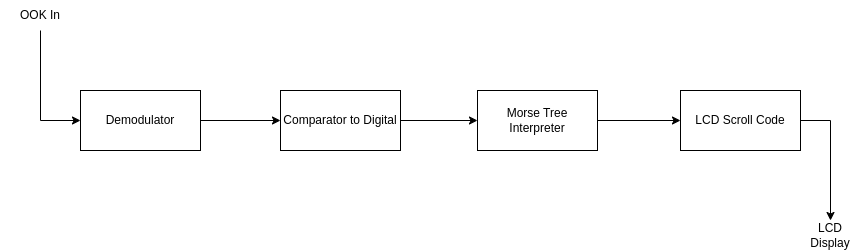
\includegraphics[width=0.4\textwidth]{images/designdiag.png}
    \caption{Morse Code Reciever Block Diagram.}
    \label{generaldiag}
\end{figure}

\section{System Design}
\subsection{Signal Demodulation}
When it comes to Morse code, the input is a form of On-Off keying, which switches on and off an oscillator depending on whether there is a binary high or low. Effectively, this is an application of the Double-Sideband Suppressed Carrier (DSB-SC) modulation scheme.

Demodulation of this to digital is very simple, and as we are working with a binary input, the demodulated waveform does not need to be perfectly coherent. A circuit diagram can be found below:

% Circuit diagram
\begin{figure}[tb]
    \centering
    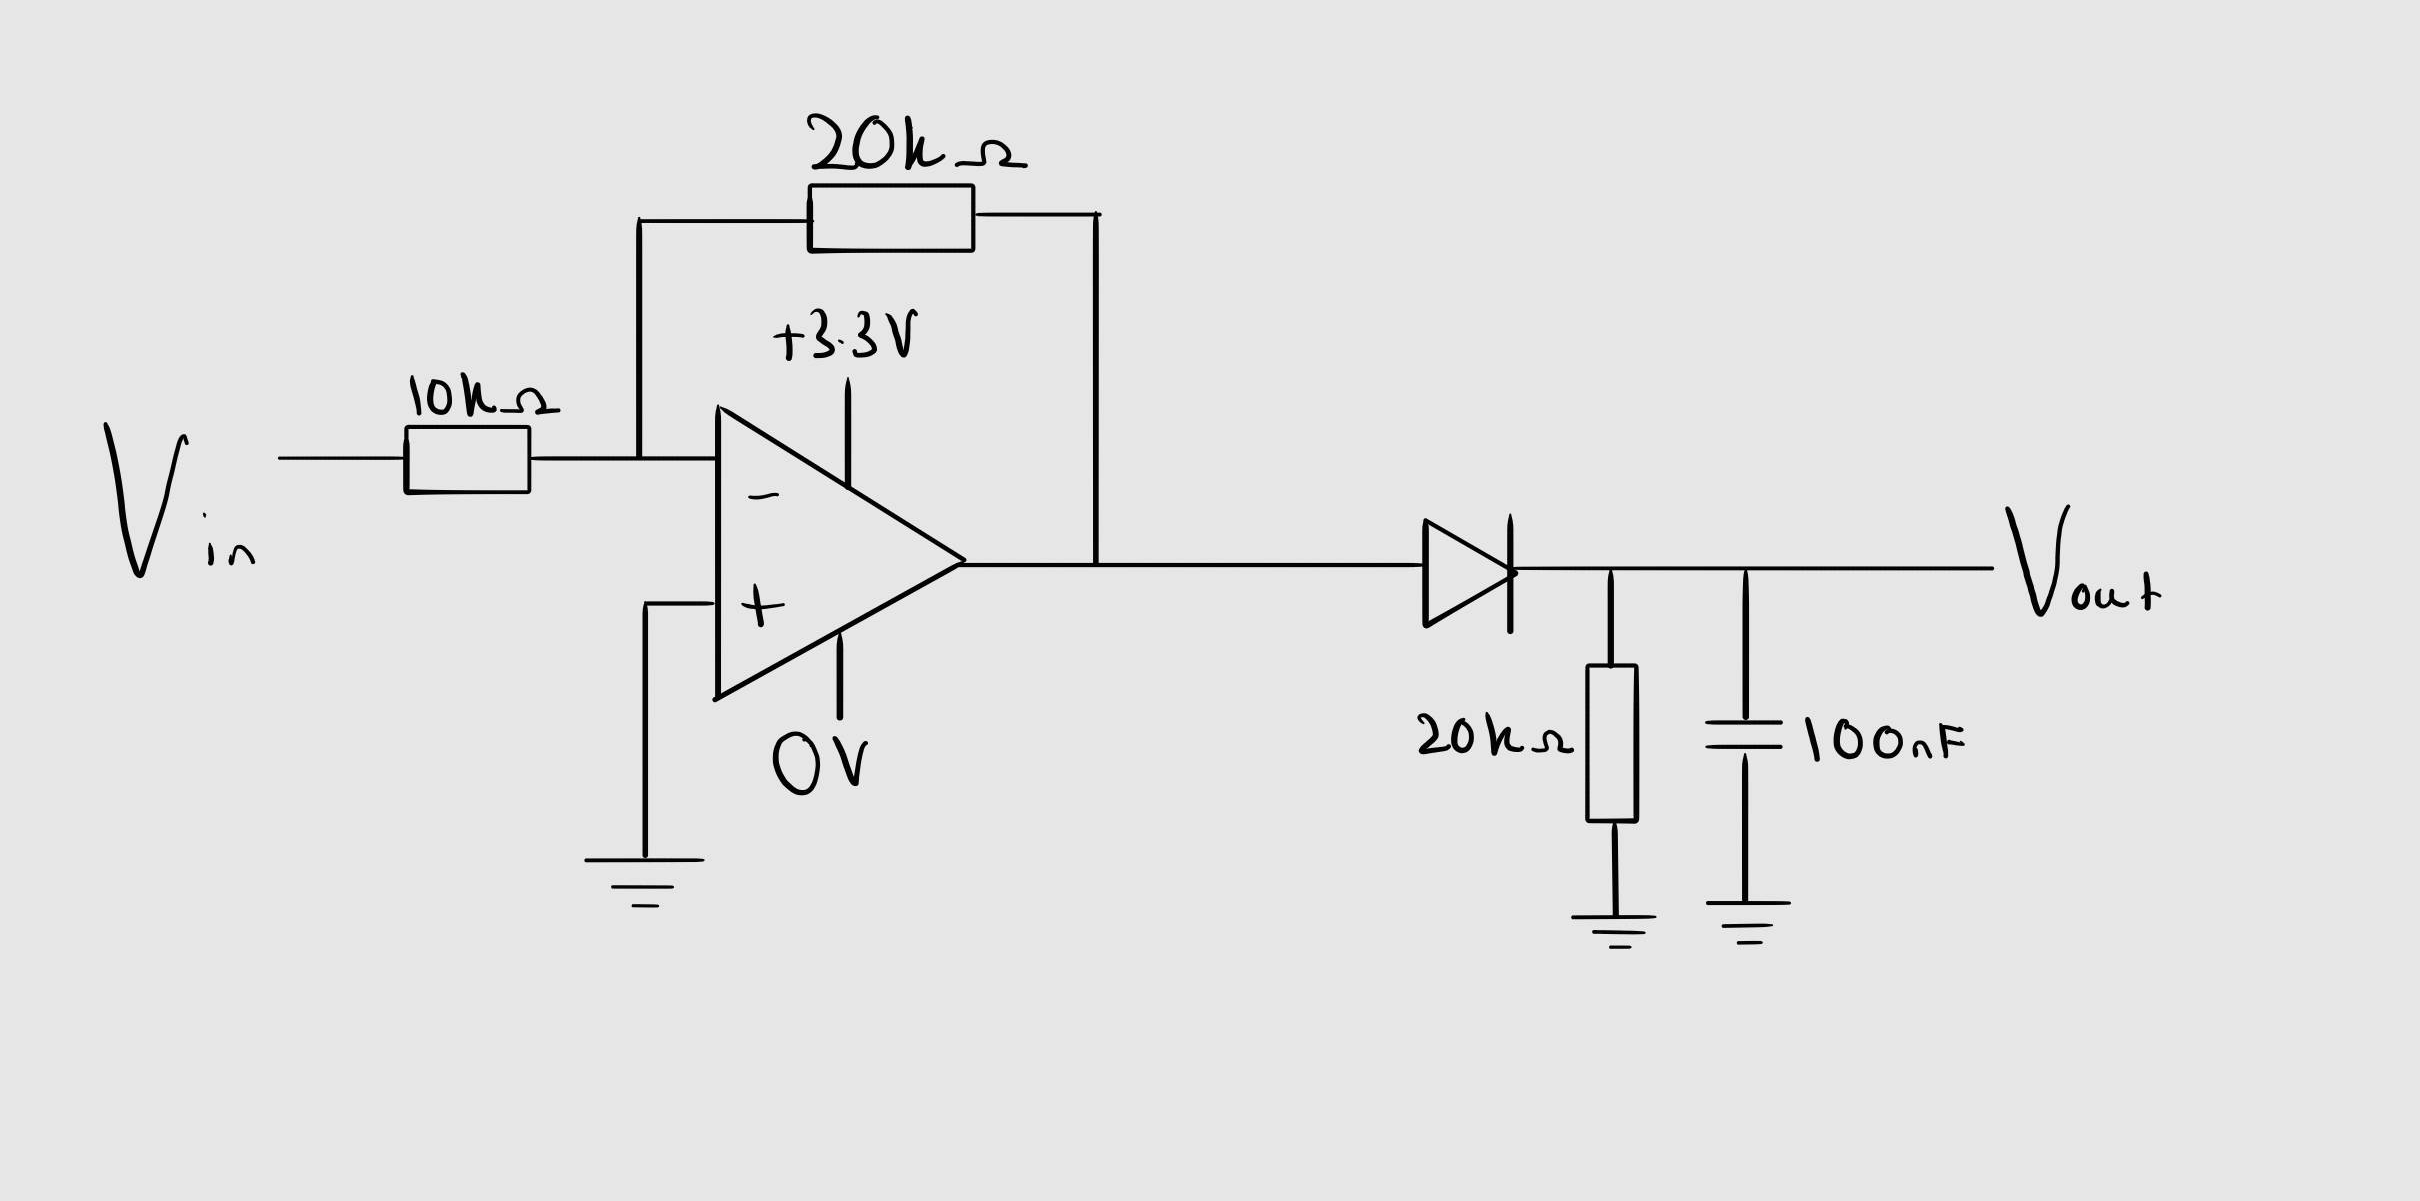
\includegraphics[width=0.4\textwidth]{images/circuit.png}
    \caption{Circuit diagram for OOK demodulation.}
    \label{whateverthehecktherefis}
\end{figure}

The above circuit, found in figure \ref{whateverthehecktherefis} has the following stages:
\begin{itemize}
\item An inverting amplifier opamp stage biased to double the amplification of the signal and limiting the voltage between $0V$ and $+3.3V$
\item a diode for rectification (can be replaced with a full-bridge rectifier if you use diodes that have a reasonable voltage drop)
\item A Resistor and Capacitor in parallel with values of $20k\Omega$ and $100nF$, respectively
\end{itemize}

\subsection{Sampling}
To sample this digital input, timers were used. This is to ensure that there is an equal $\Delta t$ between each sample, otherwise, there may be inaccuracies. To implement this, a timer was set to run every $250kHz$ [2], with the callback function set to be the comparator sample function. To allow much higher sample rates, a queue was added to act as a buffer between the sampling and processing parts. This allowed sample rates to be pushed higher. A queue size of 32 was found to be perfect. Any less would lead to dropped samples at high WPM, and any more would significantly affect system performance. An LED is used to interpret the sampled value as being high or low (green or red). This is very useful when tuning out noise.

\subsection{Binary Signal Interpretation}
Using this stream of binary samples, we can now convert the lengths of high or low periods into dashes, dots, symbol spaces, character spaces, and word spaces. To do this, every iteration of the main loop did what can be seen in figure \ref{FSM}.

% FSM diagram
\begin{figure}[tb]
    \centering
    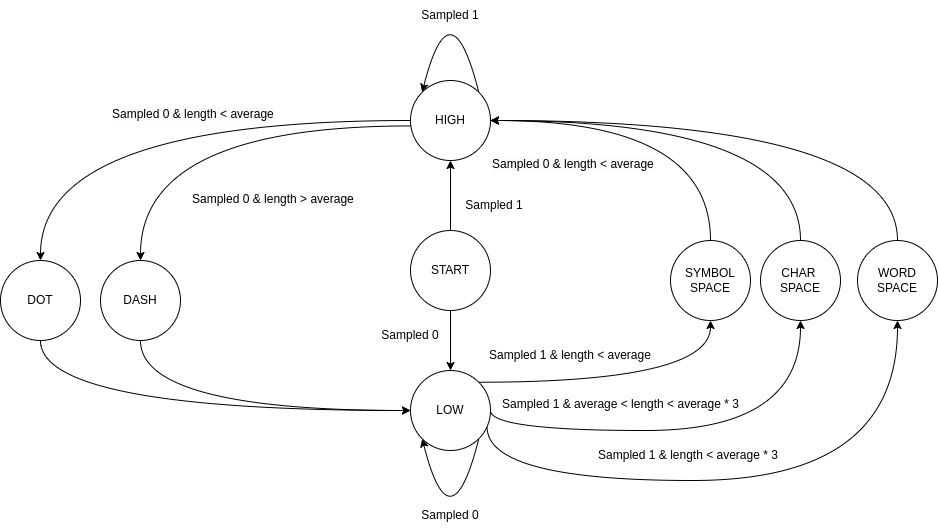
\includegraphics[width=0.4\textwidth]{images/fsm.png}
    \caption{Finite State Machine (FSM) for Morse code decoding.}
    \label{FSM}
\end{figure}

\subsection{Morse Code Translation}
Due to the binary nature of Morse code, it allows the use of a binary tree structure where each node is reachable through a dot or a dash. As seen in [1], it is intuitive that a tree of characters that are reachable using dot and dash traversals would allow for fast lookup and efficient memory usage due to the compact nature of characters, which are stored as 8 bit integers. A comprehensive binary tree that includes all necessary symbols is shown in figure 3.

% Morse code binary tree
\begin{figure}[tb]
    \centering
    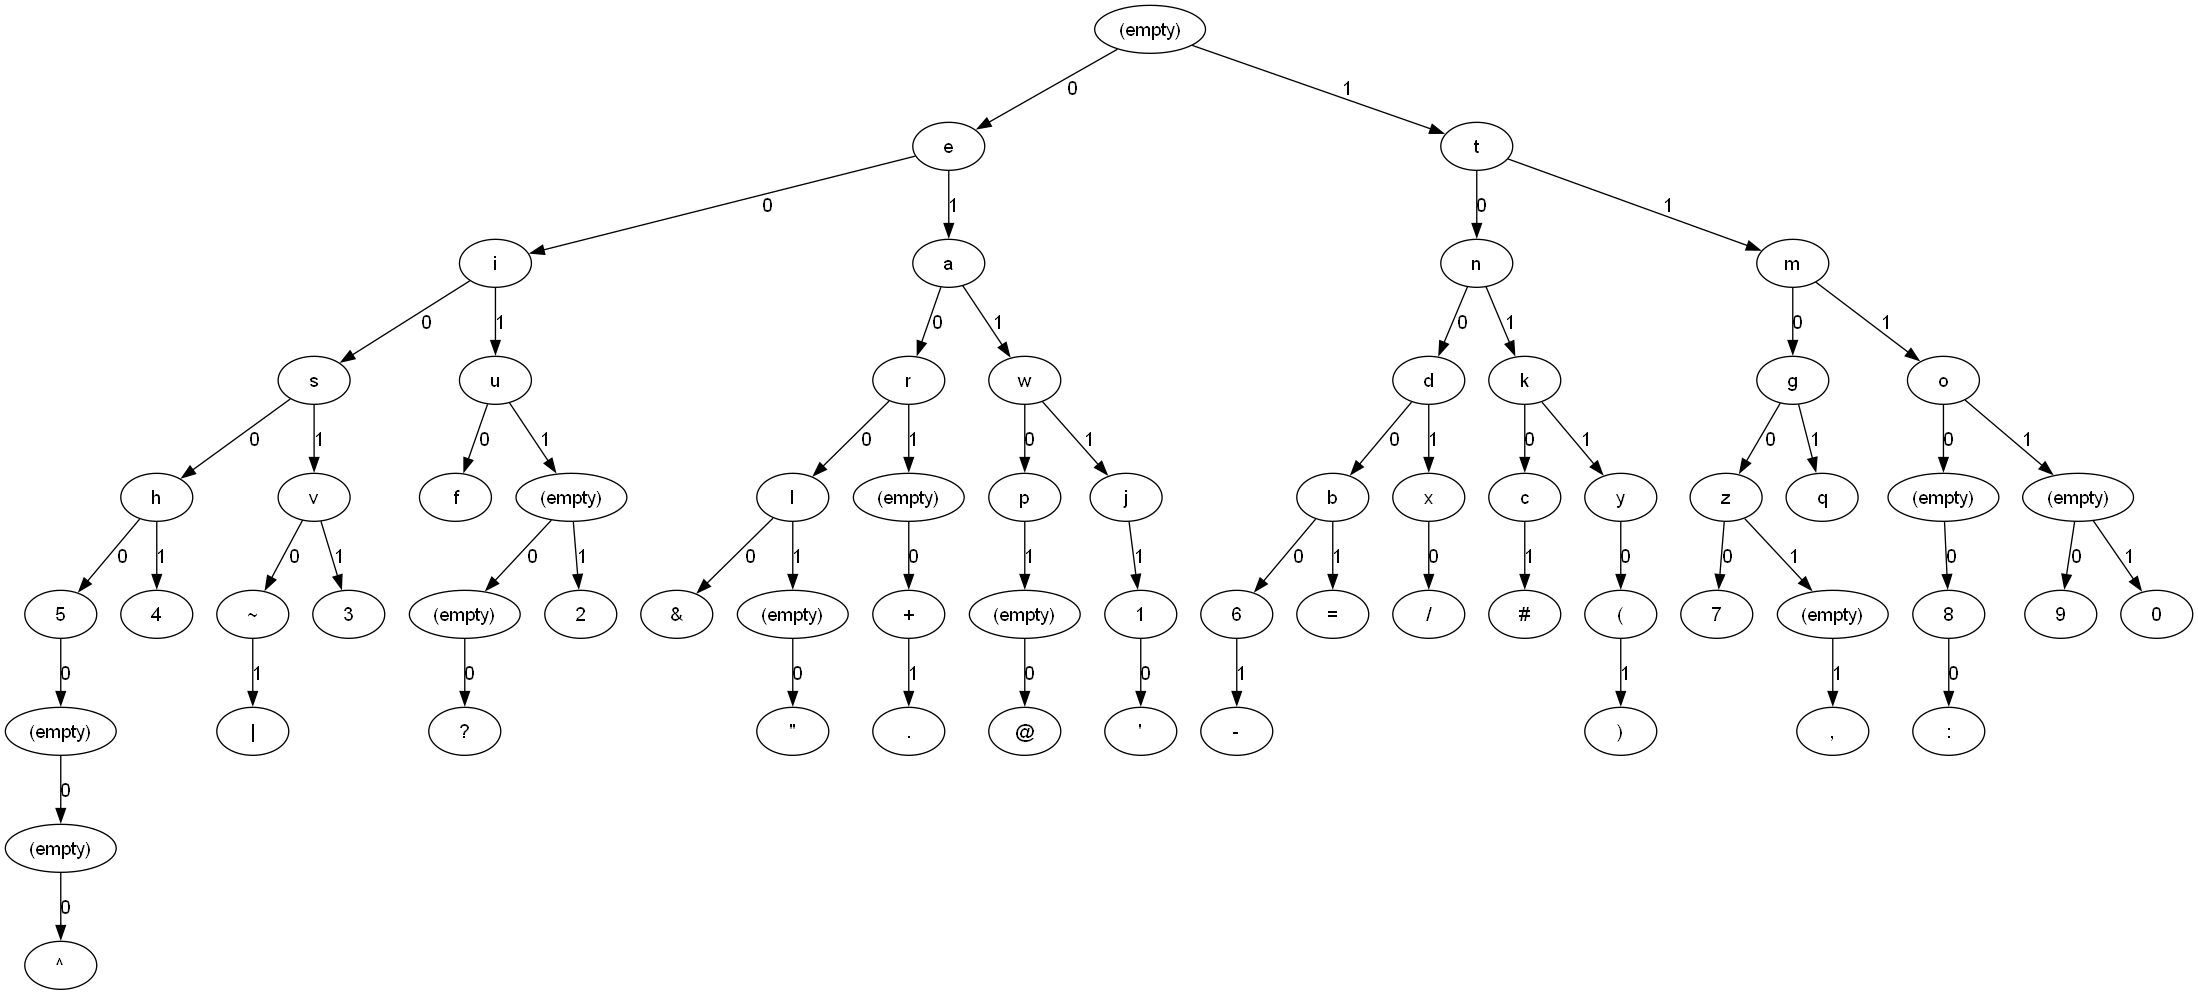
\includegraphics[width=0.4\textwidth]{images/morse_tree.png}
    \caption{Morse code binary tree.}
    \label{morsetree}
\end{figure}

\subsection{LCD Display}
To display the translated Morse signal on the LCD, predefined functions in C files from [2] are employed with adjustments and additions to engage with the functional and technical requirements of the receiver. In the case of ``lcd.c'' and ``lcd.h,'' adjustments were added to add scrolling functionality, notably in the form of a \texttt{lcd\_scroll\_char} function. This function relies on a scroll buffer for displaying the previous characters. The function checks if the output is too long to be fully displayed on the LCD’s top line, and scrolls to the left if so, making more space for the overflowing characters. This is done by checking if the number of stored characters exceeds the LCD width. If there is still room, the character is simply appended to the end, and a scroll buffer index is incremented. Once the screen real estate has been exhausted, a loop shifts all stored characters to the left to make space for the most recent one.

To fully display this output, \texttt{lcd\_scroll\_char} sets the cursor to the top left, and another loop iterates through the string buffer and outputs the sequence of characters using \texttt{lcd\_put\_char} on each element until the null terminator, filling the rest of the line with spaces if the scroll buffer is shorter than the screen.

\subsection{Merging Tree and LCD Functionality}
To merge the tree-based decoding and the functionality in the modified \texttt{lcd.c} file, header files are included in \texttt{main.c} to use vital functions such as \texttt{decodeMorse} and \texttt{lcd\_scroll\_char}. The main function code initializes a Morse buffer and index for the Morse tree, which stores a sequence of dashes (1) and dots (0) related to the current character being received. This is passed to \texttt{decodeMorse} to find the given sequence’s associated character, which is then passed over to \texttt{lcd\_scroll\_char}.

In the main code, to handle the states of the FSM, a high signal is classified into either a dot (0) or a dash (1). The element is then added to the Morse buffer. After this assignment, the buffer index is incremented by one to allocate space for the next element in the sequence to be decoded. Alternatively, the buffer index is set to 0 in the event of an overflow, but that shouldn’t occur for the receiver, as it should be able to hold all defined Morse code characters without overflow issues.

The next points in the main code showcase the seamless merging between the Morse tree code and the modified LCD code, with the ADC handling of samples. This implementation does not need explicit handling of symbol spaces, as they are simply pauses within the decoding of the same character, therefore, nothing needs to be added. In the event of a word space, the receiver checks that the Morse buffer isn’t empty, at which point \texttt{decodeMorse} decodes the last character in the word, the buffer index is reset for the next character, and \texttt{lcd\_scroll\_char} is called to display a space on the LCD to start a new word.
This analysis is applied to character spaces, the only difference being the omission of a space character to be displayed on the LCD.

Although this design easily fulfills the requirements for a reliable Morse code receiver, a switch was mapped to the modified \texttt{lcd\_clear} function as a digital input available to the user for clearing the LCD. The modified \texttt{lcd\_clear} uses a helper function, \texttt{lcd\_scroll\_reset}, which clears the scroll buffer and sets the scroll position to 0. This was added to fully comply with the functional and technical requirements.

\subsection{Multithreading}
The current system incorporates multithreading by the use of a timer structure to periodically sample the comparator input and save it to a queue [2]. The timer works by initiating an interrupt every 250 kHz to run the timer callback function, which is set to the sample function, which samples the comparator. This frequency was found to be the highest, which doesn't cause samples to be dropped, and leads to invalid outputs.

When such a timer-based interrupt is called, the infinite loop in the main thread is stopped to execute the sample function, then execution continues as normal, with the main code handling the enqueued value (assuming there aren’t any other enqueued values) in the next iteration. This approach is the only one that allows for equally time-spaced samples and does not waste system resources by waiting.

\section{Management}
Based on Fig. 1, Morse code interpretation had the first robust implementation based on the Morse code binary tree, with Akram implementing it before conversion and pause handling was determined. Initially, the task distribution consisted of Daniel implementing the sampling functionality and devising a reliable digital conversion approach with Akram, while Antoni was responsible for LCD functionality. The first reliable conversion method that was conceived was using a Goertzel’s algorithm implementation for the analog-to-digital conversion, which would then be passed onto the Morse tree. Daniel proposed a competing circuit-oriented approach, which would rely on using a physical on-off keying decoder. Although Goertzel’s algorithm was implemented and showed merit as an efficient method of finding the target tone with a capability of handling significant noise, Daniel’s approach prevailed based on its simplicity and responsible use of the limited resources of the microcontroller. The current implementation was tested with successful transmission speeds of up to 270 WPM.

Akram modified all code to remove reliance on any external libraries and merged the tree with the main code for handling dots, dashes, and pauses, with LCD function calls to display the output. Antoni and Daniel produced scrolling code to add scrolling functionality, with Antoni beginning initial LCD testing and Daniel responsible for sampling and eventually the analog to digital conversion favored over Goertzel’s algorithm. He and Akram merged this with the Morse tree and LCD functionality. Overall, the receiver easily meets all minimal requirements in addition to the functional and technical requirements. However, as a result of the robust conversion method and the rolling average threshold handling, the system has even more features, namely variable transmission speeds and noise handling. Antoni initially added scrolling functionality to \texttt{lcd\_print}, but upon testing, this seemed costly since it operated on strings and had an inefficient algorithm. Hence, Daniel implemented an independent scrolling function, \texttt{lcd\_scroll\_char}, which is the final additional feature that was added.

\section{Testing}
Before testing real-time decoding with the microcontroller, the tree was tested via unit tests, which consisted of initializing the Morse tree and passing arrays for it to decode. Assertions checked if it was the correct output and verified that the tree and decodeMorse worked reliably. As for real-time decoding, the microcontroller was tested using a variety of signals, which included:

“ABCDEFGHIJKLMNOPQRSTUVWXYZ 0123456789 .,?/'=@()-+,”
“PARIS” on loop,
“TEST,”
Random sporadic characters.

In almost all cases, there was no error in the output even up to 270WPM. Below are some images of the outputs.

% Test output (PARIS)
\begin{figure}[tb]
    \centering
    \includegraphics[width=0.4\textwidth]{images/testparis.png}
    \caption{LCD output for test string ``PARIS'' at 50WPM.}
    \label{testparis}
\end{figure}

% Test output (Alphabet)
\begin{figure}[tb]
    \centering
    \includegraphics[width=0.4\textwidth]{images/testalfabet.png}
    \caption{LCD output for test string ``ABCDEFGHIJKLMNOPQRSTUVWXYZ'' at 50WPM.}
    \label{testalfabet}
\end{figure}

In the above case, a few As were added to initialise the average.



Versioning using git for testing was essential, as it allowed tuning the code without the fear of causing irreversible bugs. With a git checkout or git pull, the latest stable version of the code could have been accessed immediately. The code was also tested with compiler optimizations at level 3, which did not cause noticeable changes, as presumably most of the processing time was I/O.

The Keil MDK debugging tool was not useful here, as the signals used needed to be real-time, which debugging was not. The microcontroller was also left on for a whole night, and then given Morse code input at the same WPM as the previous day. The receiver had to adjust in a few characters as there were a few false inputs throughout the night, but then it successfully decoded the first test string.

When adding the clear screen functionality, the computation/waiting of i/o was noticeable. The check to see if the switch is high or low reduced the maximum WPM of the system from 300WPM to 270WPM. Using “PARIS” as a reference, Morse input with 50 dots, this translates to 225 dots per second, or 1 dot roughly every 4.4 microseconds. This exceedingly fast transmission rate indicated that our receiver design uses the memory and CPU of the LPC4088 resourcefully with fast interrupt responses and robust decoding logic. Given our design and the CPU’s clock speed of 120 MHz \cite{lpc4088oem}, the receiver excelled at standard rates such as 50 WPM, which do not push the microcontroller anywhere near its limits.

\section{Closure}
After extensive testing of the receiver, the system yielded exceptional results, easily fulfilling several additional requirements stated in the assignment specifications. The system could target a wide variety of frequencies, decoded reliably under extremely noisy conditions, and reached transmission speeds that made inputs unintelligible to the human ear. The current world record for Morse code transmission was set by Andrei Bindasov at 230 Morse code marks per minute (dashes or dots per minute) [3]. Our receiver was able to receive more words per minute than the world record holder sent in marks per minute, easily exceeding any conceivable human transmission rate. The microcontroller is likely to go much further in WPM if the I/O time were shorter.

Although the final system was desirable, the initial planning and development of the receiver deviated from our expected timeline, and the task distribution was handled more flexibly than anticipated, although the task independencies were still clearly outlined. Unfortunately, it took some time to adopt Keil MDK for remote testing and development. After Keil was set up successfully, development moved at a significantly smoother and more productive pace. Each component of our receiver was designed with modularity in mind. A minor limitation of our receiver was that it omitted the final character in the stream. However, this can be easily circumvented by sending another character.

% Dummy citation to avoid "no \citation commands" warning
\nocite{itu}

\begin{thebibliography}{9}

\bibitem{itu}
ITU, International Morse Code. ITU-R Recommendation M.1677-1, Oct. 2009. [Online]. Available: \url{https://www.itu.int/rec/R-REC-M.1677-1-200910-I/}

\bibitem{umcode}
“Code,” University of Malta CCE2014 Course

\bibitem{morseworldrecord}
Morse code world record. [Online]. Available: \url{https://www.guinnessworldrecords.com/world-records/fastest-speed-for-a-morse-code-transmission}

\bibitem{lpc4088oem}
Embedded Artists, “LPC4088 OEM Board.” [Online]. Available: \url{https://www.embeddedartists.com/products/lpc4088-oem/} [Accessed: May 31, 2025].

\end{thebibliography}

\end{document}
